\chapter{Background}
\label{ch:background}

This section presents background information of the technologies and hardware used in this project. First, an introduction of RFID is provided in Section \ref{sec:rfid}. This includes a description of the technology, typical components of such systems, and potential applications in the context of this work. Then, Section \ref{sec:rssi} discusses the Received Signal Strength Indicator (RSSI) as the metric for measuring distance between readers and tags. Next, the hardware components of the project are presented in Section \ref{sec:projhard}. These are RFID readers, an active tag, and single-board computers (Raspberry Pis). Section \ref{sec:locprinc} includes a discussion of general localisation principles and challenges. This chapter is concluded by a survey of previous work using active RFID components to localise objects in indoor environments.

\section{Radio Frequency Identification (RFID)}
\label{sec:rfid}

Radio Frequency Identification (RFID) is a wireless technology that communicates electronically stored data between radio devices. This information is used to remotely identify objects marked with tags \cite[p. 5]{Hunt2007}. RFID uses electromagnetic waves to carry information. Such systems differ from each other by their radio frequency of operation, physical coupling method, and transmission range \cite[p. 21]{Finkenzeller2010}. Radio frequencies used in RFID range from 100kHz to 10GHz \cite{Landt2005}. The physical coupling methods in RFID classify such systems into three main categories. Close-coupling systems have a small interrogation range of up to 1cm. Remote coupled systems are capable of sensing information of up to 1m. All systems that can wirelessly read data from a marked object positioned over 1m away are called long-range systems \cite[p. 22]{Finkenzeller2010}. A RFID system has three compulsory hardware components, tags (also known as transpoders), readers (also called interrogators), and controllers.

\subsection{RFID tags}

A tag is a data-carrying device that transmits identification information in response to a received signal from a reader. RFID tags usually consist of an antenna attached to a microchip \cite[p. 2]{Want2006}. The hardware can be encapsulated in different types of enclosures. Tags come in different shapes and sizes depending on their operational environment (Figure \ref{fig:rfidtags}). RFID tags also have memory where the identification and sometimes additional information is stored. Additional data might include a delivery date of a parcel, for example. The information stored on a tag is usually only for reading. However, there are implementations of the RFID technology that benefit from writing data to a tag. For instance, a pallet might have a tag attached to it that can store the contents of the pallet as it changes over time \cite[p. 8]{Hunt2007}.

\begin{figure}
	\begin{center}
		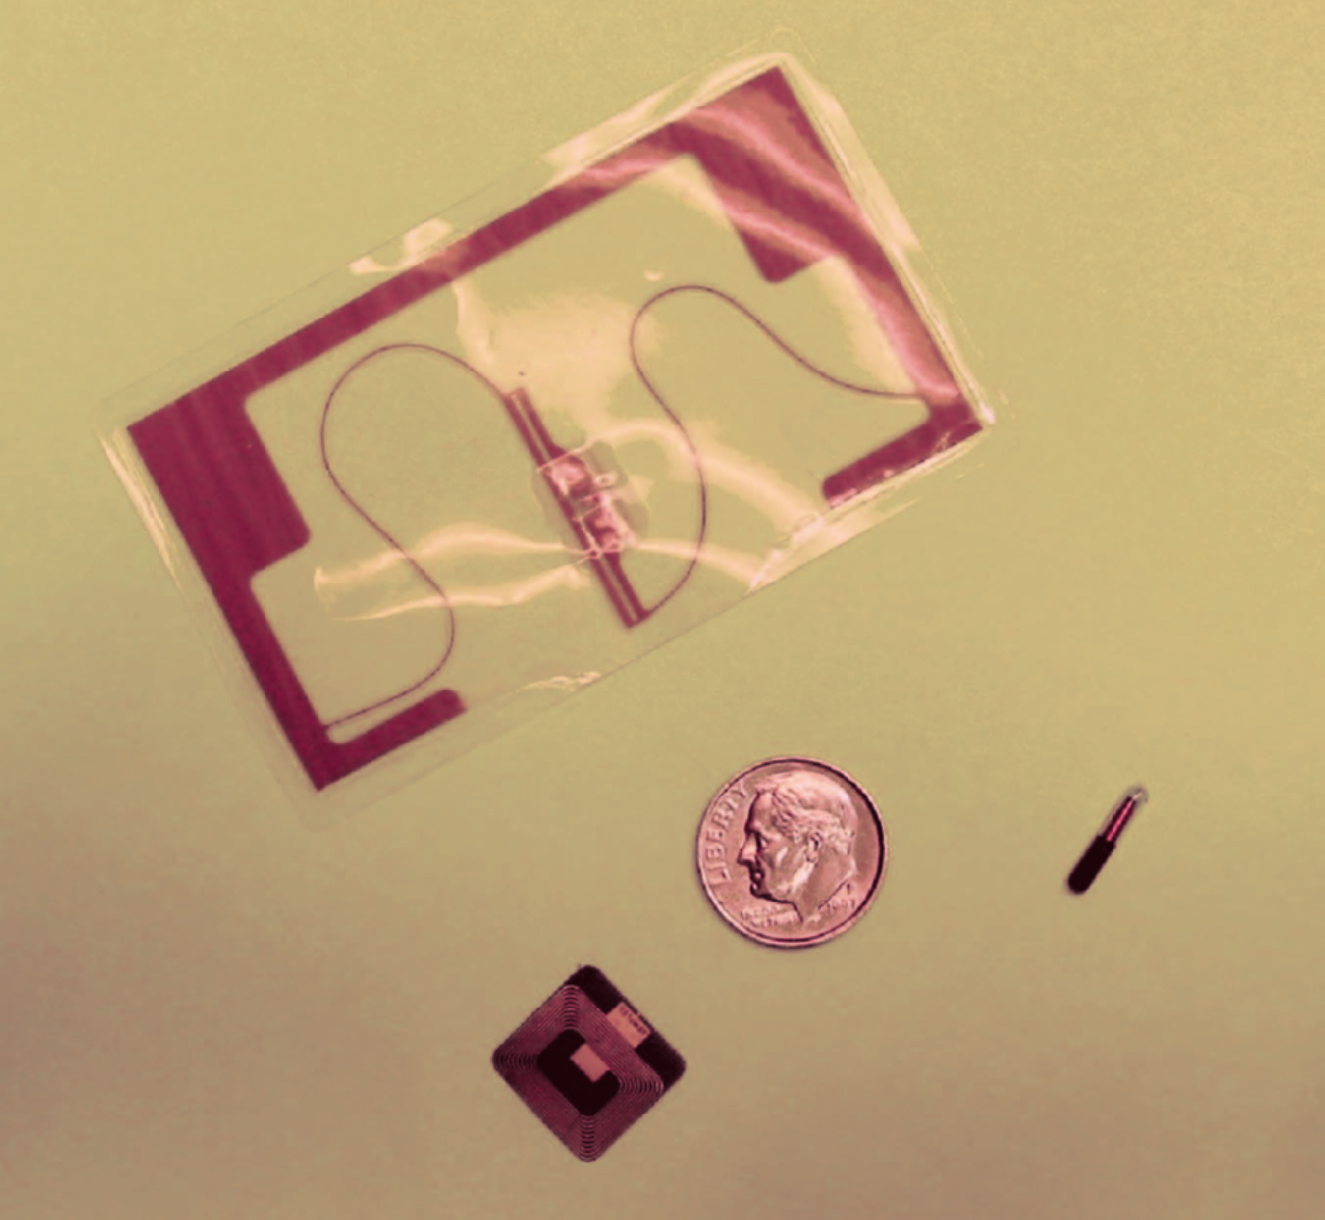
\includegraphics[width=0.5\textwidth]{figures/rfidtags}
		\caption{Three different variants of RFID tags. Figure from \cite{Want2006}.}
		\label{fig:rfidtags}
	\end{center}
\end{figure}

\subsubsection{Passive and active tags}

Tags can be classified into two main categories, passive and active . Passive tags do not require a power source. They communicate with readers by reflecting part of received radio waves, a term referred to as backscatter modulation \cite{Bolic2010}. They have a number of advantages, which include their small size, very long operational life, and low price. Nevertheless, passive tags need to be in the readers' range in order to operate. This is because passive tags obtain the power they need to supply their circuitry from an electromagnetic signal received from a RFID reader. A charge builds up into a capacitor that can power the passive tag and transmit the identification information it is storing \cite{Weinstein2005}.

In contrast, active tags require a power source in the form of a battery or are directly connected to the electrical grid \cite{Want2006}. Although, their lifetime might be limited by the available energy, active tags can be read from greater distances compared to passive tags. This is because they have their own power source which enables them to emit strong signals to the readers \cite{Weinstein2005}. Compared to passive tags, active ones are larger in size and have a higher price.

\subsection{RFID readers}

A reader is a radio device that is capable of transmitting interrogation signals and capturing information send back by tags. The reader's transmission frequency specifies the operational frequency of the RFID system, which also defines their practical reading range \cite{Finkenzeller2010}. These devices usually consist of a radio frequency (RF) module, that is capable of sending and receiving  signals, an antenna, and a control unit in the form of a microprocessor. RFID readers have the following main functions:

\begin{itemize}
	\item read/write data from/to a RFID tag,
	\item power a passive tag,
	\item relay the obtained information to a host computer \cite[p. 9]{Hunt2007}.
\end{itemize}

Readers are responsible for bringing additional functionality to a RFID system. This includes support for simultaneous sensing of multiple tags, authentication of tags to prevent unauthorised access to a system, and data encryption of the stored data to ensure integrity \cite[p. 10]{Hunt2007}. There are a wide range of RFID readers that differ in their operational radio frequency, range, and coupling method. These properties are formed by factors such as the specifications of the system, its budget, and security requirements \cite[p. 25]{Finkenzeller2010}.

\subsection{RFID controllers}

The third component of a RFID system is the controller or server. It is a computer that is responsible for connecting and communicating with multiple readers, aggregating any incoming data, and processing it. Readers can be connected to the server using a network or serial connection. Identification information is usually stored in a database and is used by an application software \cite[p. 11]{Hunt2007}. Figure \ref{fig:rfidsys} shows the components of a typical RFID system.

\begin{figure}[h]
	\begin{center}
		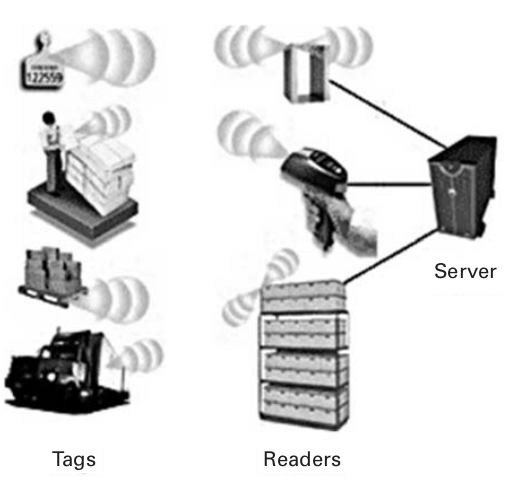
\includegraphics[width=0.5\textwidth]{figures/rfidsys}
		\caption{Components and applications of RFID. Figure from \cite[p. 20]{Rida2010}.}
		\label{fig:rfidsys}
	\end{center}
\end{figure}

\subsection{RFID applications}

RFID hardware is becoming more inexpensive, which creates a wide range of possible scenarios where this technology can be applied \cite{Nath2006}. The most widespread applications are in tracking of objects or people, in supply chain and asset management, and in health services \cite{Weinstein2005}.

Passive RFID systems can be used as an alternative and improvement of the current standard for identification of products, the barcodes.  Reading a barcode attached to an object requires a direct line of sight between a reader and a tag. In addition, barcodes can get obscured by other objects or substances, which hinders the identification process. RFID solves these disadvantages. A line of sight is not required when reading data from tags attached to objects. RFID tags also support a larger set of unique IDs compared to bar codes, can be reprogrammed, and can store additional data depending on the application requirements \cite{Weinstein2005}.

In the context of this project, which is concerned with location sensing, RFID has applications in tracking important objects or personnel and trying to pinpoint their position. For example, active RFID systems can be used in hospitals to monitor the location and life cycle of patients in an indoor environment \cite{Cangialosi2007}. Expensive hospital equipment could be tracked so that it would be at the right place and time. Another possible scenario is to track school kinds while on school grounds in order to find lost children and monitor their attendance \cite{Swartz2004}.

\section{Received Signal Strength Indicator (RSSI)}
\label{sec:rssi}

Some RFID readers provide an indication of the strength of radio signals received from tags. This metric is called Received Signal Strength Indicator (RSSI). Its value is often output along with the identity information stored in a tag. It is estimated at the reader side before amplifying the received input. RSSI is an uniteless measurement of the power of the received signal represented as a positive value with certain resolution range. A resolution of two bits gives a precision of eight possible values for RSSI. This means that there are eight different steps of estimating how far a tag is. A resolution of eight bits, supported by the project hardware, lets readers output values between 0 and 255 giving a better approximation of the distance between a reader and a tag. 

\subsection{RSSI and RSS}

RSSI is not to be confused with the Received Signal Strength (RSS), on which RSSI is based. RSS is usually measured in dBm\footnote{dBm - Power ratio in decibels of power referenced to one milliwatt (mW) - \url{http://en.wikipedia.org/wiki/DBm}}. It represents the attenuation of a received signal and is a function of the distance between a receiver and transmitter \cite{Bouet2008}. In WiFi, the 802.11 standard does not define the relationship between RSSI values and reported signal power levels. It is up to the manufacturers to provide a conversion function or table that specifies range and accuracy of the RSS values and how these translate into a RSSI range between zero and a maximum value \cite{Lui2011}. The above applies to RFID, which is also a radio technology. 

\subsection{RSSI and distance}

A third relationship is the one between RSSI and distance. In other words, it is the problem of using RSSI reader measurements to estimate the distance separating a receiver and transmitter. More importantly, one might ask whether RSSI is a reliable parameter for localisation algorithms in wireless networks. This is not the main question that this work is concerned with. However, the reliability of this measure is of prime importance because position estimation here relies solely on this parameter. 

On the one hand, there are studies that test the reliability of both RSS and RSSI for location sensing \cite{Elnahrawy2004, Parameswaran2009}. These concluded that the limitations of determining inter nodal distances are fundamental. On the other hand, signal strength is readily available in devices today, which creates attractive opportunities for estimating position without any additional hardware. Indeed, there are a number of WiFi-based systems that rely on received signal strength including the Horus WLAN location system \cite{Youssef2005}, the EZ localisation system \cite{Chintalapudi2010}, an indoor location system using trilateration \cite{Cook2005}.

\subsection{How RSSI fits in this project}

Although RSSI is not considered a reliable measure for distance due to the physical properties of radio waves and due to cluttered and dynamic indoor environments, the aforementioned systems show that researchers and engineers try to get the best of what is already provided. In the same manner, this work uses RSSI reader measurements as a basis for location sensing. This is done using a translation table that converts RSSI into a distance metric. The methods used and the challenges faced while doing this are explained in ... FILL CHAPTER AND SECTION.

\section{Project Hardware}
\label{sec:projhard}



\subsection{RF9315R-u Active RFID 8 Meters Receiver with RSSI Module}

\subsection{RF8315T Active RFID 8 Meters Transmitting Module}

\subsection{The Raspberry Pi}

A single-board computer is a computer that is built on a single circuit board. It features most of the components of a personal computer. It has a processor, memory, storage, different microprocessors, and input/output interfaces. The Raspberry Pi is a particular implementation of a single-board computer. Figure \ref{fig:raspi} shows a graphical representation of its main components. Some of its strengths directly relating to this project are that it:
\begin{itemize}
 	\item has an affordable price that ranges from 25 to 35,
 	\item can be connected to a RFID reader through USB or GPIO pins,
 	\item is credit-card sized,
 	\item consumes little power (3.5 W).
\end{itemize}

\begin{figure}[h]
	\begin{center}
		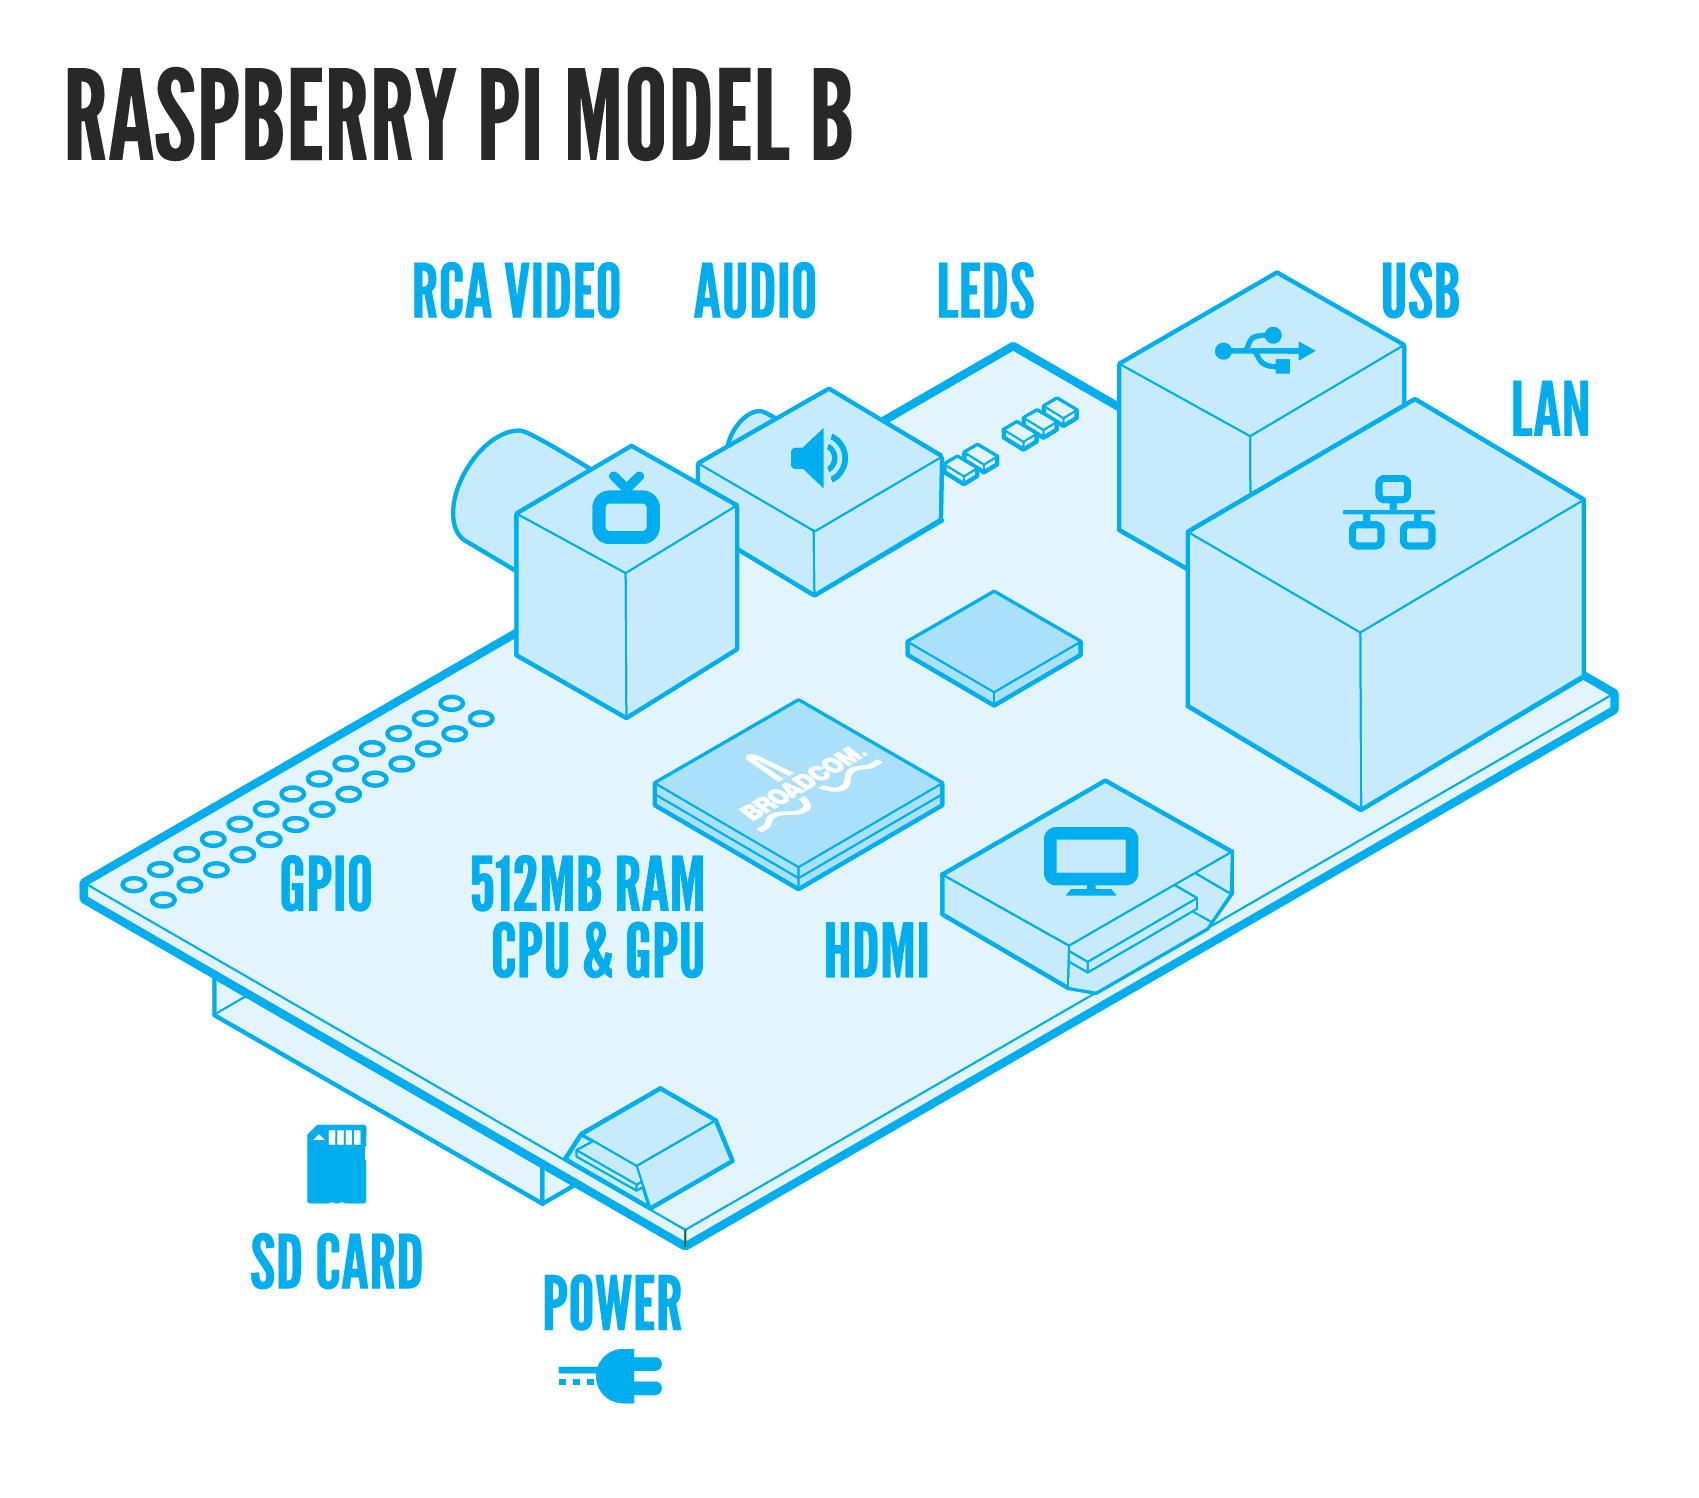
\includegraphics[width=0.6\textwidth]{figures/raspi}
		\caption{Raspberry Pi Model B. Figure from \url{http://www.raspberrypi.org/faqs}.}
		\label{fig:raspi}
	\end{center}
\end{figure}


\section{Localisation principles}
\label{sec:locprinc}

Using the distances between readers and a tag, this project will employ the geometrical process of trilateration. It determines the relative position of a tag using properties of circles. The distance from a reader to a tag is the radius of a circle that could be drawn around the reader. The intersection of circles of three readers can be used to determine the approximate location of a tag relative to the readers. This technique has practical applications in surveying and navigation. Figure \ref{fig:lat} shows the concept of trilateration applied in the setting of this project.

\begin{figure}
	\begin{center}
		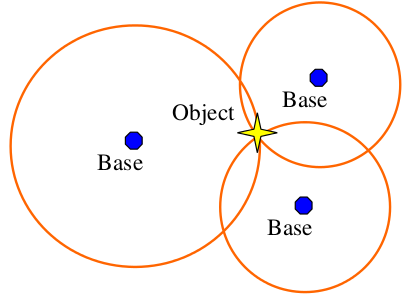
\includegraphics[width=0.45\textwidth]{figures/lateration}
		\caption{The trilateration geometrical process applied in the context of this project. Figure from \cite{Hightower2000}.}
		\label{fig:lat}
	\end{center}
\end{figure}

\section{Previous work}

\textbf{Copied from IRP.}

\subsection{SpotON}

SpotON is localisation algorithm based on lateration with distance estimation using RSS measurements. SpotON's operation involves a number of readers collecting signal strength information from active tags to determine their positions in the 3D space. At the time or their research, Hightower and his colleagues were using RFID hardware with 2-bit accuracy when measuring received signal strength \cite{Hightower2000}. They identified that this accuracy is not enough to achieve the precision required for localisation in small indoor environments. The authors mentioned that 8-bit accuracy (from 0 to 255) could be used in the future for improved results \cite{Hightower2000}. The SpotON algorithm consists of two main parts. First, RSS measurements are converted into a distance estimation. This is done using a translation function relying on numerical variables that were identified based on observation. This function is not generic and probably cannot be applied in this project. However, it will be analysed because it might provide important information about the relationships between RSS and distance. The next part of the algorithm is to apply a localisation algorithm that tries to minimise RSS errors \cite{Hightower2000}. It is based on the lateration geometrical process to estimate a position for an active RFID tag. This project will be using some of the methods and procedures applied in the SpotON system.

\textbf{Copied from project progress.}

It is a fine-grained tagging technology for 3D location sensing using radio signal strength analysis. They tried to develop a low cost system compared to commercial solutions available at their time. They believe that the accuracy and efficiency of location sensing could be enhanced by sensor fusion, i.e. adding more sensors (accelerometers) and building maps. These authors talk about ubiquitous computing. They try to separate the meanings of positioning and tracking. Positioning is concerned with providing means to calculate location which can be used to compute an actual position. Tracking is monitoring objects without involving them in the computation. They define location sensing to be such systems that separate the manipulation of location data from the mechanisms of actually pinpointing the objects. They used radio devices with a serial connection similar to the devices that will be used in this project. They were talking about the limitations of such a serial connection (R232) which will mitigated in our case by using a converter from serial to USB. In our case base stations that aggregate information and a server that processes it is combined into the Raspberry Pi computer. 
	
This paper summarises the localisation algorithm they used based on the conversion of distance into signal strength in 6 directions in 3D. Then the measured RSS is compared to the 6 known RSS to find a location around a reader. They do not store data or timing information on the server, which I am planning to do. They have a visualisation client written in OpenGL. 
	
Their results are not very accurate because they use radio devices with 2-bit RSS accuracy compared to modern onces with 8-bit accuracy. Their second problem was measurement frequency which happened between 10 to 20 seconds, which is too slow to monitor real-time position changes of objects. They identified these limitations and solved them by creating a custom hardware.

\subsection{An Introduction to RFID Technology \cite{Want2006}}

\textbf{Copied from project progress.}

Read and highlighted "An Introduction to RFID Technology" by Roy Want \cite{Want2006}. It is good introductory article that clearly explains different classifications of RFID. It has helpful graphics for the distinction between near and far field RFID communication.

\subsection{RFID Tags: Positioning Principles and Localization Techniques \cite{Bouet2008}}

Contains similar introduction to RFID technology. Explains the role of the server (RasPi in our case) connected to the readers that runs a localisation algorithm and provides the middleware for communication between servers. Contains a good classification of indoor localisation algorithms - distance estimation, scene analysis, and proximity. A brief but clear explanation of lateration with a useful figure. Contains a classification of range measurements techniques starting with Received Signal Strength (RSS) that will be used in this project. "The attenuation (gradual loss) of emitted signal strength is a function of the distance between the emitter and the receiver."

A classification of different RFID localisation schemes is proposed. The first one is SpotON where multiple readers collect RSS measurements in order to approximate distance from the tag. Then lateration is performed to localise the tag. 
	
Landmarc is another approach that uses reference tags that are regularly deployed on the covered area. The idea here is to select the k nearest reference tags that are closest to the unknown tag using differences in RSS measurements. Having identified the k nearest reference tags their coordinates are used to localise the unknown tag. 
	
VIRE extends the methods used in Landmarc by defining a proximity map that every reader records. This proximity map consists of a 2D grid of reference tags where the centre of a cell is a tag. The difference in the RSS measurements between reference and unknown tag helps label cells in the proximity map so that it can be constructed. The union of individual proximity maps gives a global proximity map for the unknown tag.
	
Simplex is a method that requires different transmission power levels. I am not sure if our equipment has this feature.
	
A Kalman filtering method is briefly explained but have to read the original paper because it is hard to understand from a one paragraph description of the method.
	
Scout is a probabilistic localisation technique that uses a probabilistic RSS model to estimate distances from a tag to readers. Predicted beliefs are calculated and corrected using reference tags until a good model is constructed.

\subsection{Semantic Sensor Net: An Extensible Framework\cite{Ni2005}}

It is more concerned with sensor networks with multiple nodes, where the nodes have less importance than traditional computer networks. The article proposes an extensible framework for sensor networks that relies on attaching semantics (meanings) to sensor data but also to sensor nodes, location, context, and queries. The idea is to attach a meaning to every piece of information so that those meanings can be used by the network to route and aggregate data more efficiently, for example. This paper does not have a direct connection to this project but gives grounds for thoughts about attaching meaning to measurements, considering heterogeneous RFID reader nodes, and taking scalability into account.

\subsection{LANDMARC: Indoor Location Sensing Using Active RFID \cite{Ni2004}}

LANDMARC is a location sensing system that uses RFID for locating objects inside buildings. Its major advantage is that it improves the overall accuracy of locating objects by using reference tags. They believe that the choice of technology and techniques is of crucial importance for the granularity and accuracy of the location information. They identify that range of a RFID system is determined by the power available at readers and tags and the environmental conditions and structures. In free space, the signal strength reduces in inverse proportion to the square of the distance. They found out that instead of using a lot of readers, they can arrange a number of tags in a 2D rectangular grid to use as reference tags. They associate reference tags with landmarks that help navigation in a city, for example. The advantage is that tags are cheaper and are subject to the same environmental factors as the tags being tracked. The authors believe that the placement of readers and reference tags is very important for the accuracy of the system. They needed an algorithm to connect the relationships between signal strengths and power levels that the readers return.
	
Their setup consists of RF tags and readers with a wireless module for communicating measurements to a location server. Their methodology is explained very good in their paper and relies on Euclidean distance between reference tags and unknown tags and also on k nearest neighbours to pinpoint a possible position. They apply a weighing factor when computing coordinates. To measure the accuracy of the system error distance is used. It is the linear distance between real coordinates and computed coordinates.
	
They discuss different parameters of the system. First, they found through experimentation that 4 nearest neighbours provide the best results during most of their tests. They also acknowledge the environmental factors night vs. day tests, change of placement of the tracking tags. They have restricted the number of readers used but point out that more readers provide better accuracy in certain cases. The LANDMARC system is based on reference tags so the authors discuss in detail the placement and number of the reference tags. They argue that density of reference tags plays an important role for the accuracy of the system. A good setup, they used, was consisting of 4 readers and 1 reference tag per square meter resulting in an average distance error of 1 meter.
	
Back in 2004 when the paper was written, the authors identified the hardware problems of the current RFID technology. None of RFID products supplied signal strength directly which requires unnecessary processing and sacrifice of accuracy. They also were complaining about the long latency between actual placement of tracking tags and the system computing their location. Two factors were contributing to this problem. One being the scanning time of the readers, not supporting RSS. The second the time interval of a tag emitting its ID, which is not a configurable parameter. They also identified different power levels detected by a reader from two tags which resulted in variation in their behaviour.

\subsection{Location Estimation Technique using Extended 3-D LANDMARC Algorithm for Passive RFID Tag \cite{Khan2009}}

It is an extension of LANDMARC for 3D. They used passive instead of active tags. They use RSSI which is availble from the readers they used instead of computing it from power levels. The error rate they recorded was 0.5m when estimating location. The authors explain what RSS is and summarise relationships between RSS values and distance metrics for outdoor and indoor environments. They explain that RSS measurements may suffer from multi-path fading, shadowing, diffraction, reflection, and scattering. They explain what scene analysis (finger printing) is and the two phases it consists of (offline and online). They summarise the main methods used with scene analysis: probabilistic, kNN, and neural networks. They use the same methodology as the original LANDMARC system but extend it to 3D, adding 'z' coordinate. For their experiments they used 3 readers, 2 tracking tags, and 11 reference tags. They supply all their intermediate and final results in tables with computed values for RSS tag vectors, Euclidean distance between reference and tracking tags, weights for every distance, reference tags coordinates, and estimated tracking tag's coordinates.



\section{Summary}
